\documentclass[a4paper,ngerman, 11pt, DIV11]{scrartcl}
%\documentclass[a4paper,ngerman, 11pt, pagesize]{report}

%% Päambel
\usepackage[T1]{fontenc}
\usepackage[utf8]{inputenc}
\usepackage{babel}

\usepackage{cite}
\usepackage{xcolor}
\newcommand\Diskussionspunkt[1]{\textcolor{red}{#1}}
\usepackage{ulem}

\usepackage{url}
% keine rote Rahmen um die Links anzeigen
\usepackage[pdfborderstyle={/S/U/W 0}]{hyperref}
%\usepackage{hyperref}

% Grafikpaket laden
\usepackage{graphicx}

% Tabellen
\usepackage{booktabs}
\usepackage{longtable}

% pdf einbinden (A3)
\usepackage{nextpage}
\usepackage{afterpage}
\usepackage{pdfpages}
\usepackage{typearea}
\usepackage{pdfpages}

\usepackage{lscape}


% Quelltext
\usepackage{listings}
 \usepackage{color}
 
 \definecolor{middlegray}{rgb}{0.5,0.5,0.5}
 \definecolor{lightgray}{rgb}{0.8,0.8,0.8}
 \definecolor{orange}{rgb}{0.8,0.3,0.3}
 \definecolor{yac}{rgb}{0.6,0.6,0.1}
 
  \lstset{
   basicstyle=\scriptsize\ttfamily,
   keywordstyle=\bfseries\ttfamily\color{orange},
   stringstyle=\color{green}\ttfamily,
   commentstyle=\color{middlegray}\ttfamily,
   emph={square}, 
   emphstyle=\color{blue}\texttt,
   emph={[2]root,base},
   emphstyle={[2]\color{yac}\texttt},
   showstringspaces=false,
   flexiblecolumns=false,
   tabsize=2,
   numbers=left,
   numberstyle=\tiny,
   numberblanklines=false,
   stepnumber=1,
   numbersep=10pt,
   xleftmargin=15pt
 }


%%  Variablen
\newcommand{\authorName}{Ladina Bilgery \and Thomas Wieling}
\newcommand{\auftraggeber}{Interessengemeinschaft Wetterstation Arbon}
\newcommand{\auftragnehmer}{Interstaatliche Hochschule für Technik NTB}
\newcommand{\projektName}{Multiplattform-fähiges und barrierefreies User Interface und Datenmanagement für die Wetterstation Arbon}
\title{\projektName~(Bachelorarbeit)}
\author{\authorName}
\date{\today}

%%  Create a shorter version for tables. DO NOT CHANGE 
\newcommand\addrow[2]{#1 &#2\\ }
\newcommand\addheading[2]{#1 &#2\\ \hline}
\newcommand\tabularhead{\begin{tabular}{lp{13cm}}
\hline
}
\newcommand\addmulrow[2]{ \begin{minipage}[t][][t]{2.5cm}#1\end{minipage}
   &\begin{minipage}[t][][t]{8cm}
    \begin{enumerate} #2   \end{enumerate}
    \end{minipage}\\ }
\newenvironment{usecase}{\tabularhead}
{\hline\end{tabular}}


% damit Bilder im aktuellen Kapitel dargestellt werden
\usepackage{placeins}
\usepackage{geometry}



%%  Beginn Dokument
\begin{document}
\pagenumbering{roman}
\begin{titlepage}
\maketitle
\thispagestyle{empty} 

\begin{verbatim}

\end{verbatim}


  \begin{tabular}[t]{ll}
	Projekt:       & \quad \projektName \\[1.2ex]
	Auftraggeber:  & \quad \auftraggeber\\[1.2ex]
	Auftragnehmer: & \quad \auftragnehmer\\[1.2ex]
  \end{tabular}

\begin{tabular}{|p{3 cm}|p{3 cm}|p{5 cm}|}
\hline
\textbf{Version} & \textbf{Datum} & \textbf{Autor(en)} \\
\hline
\hline
1.0 & 16.11.2017 & \authorName \\
\hline
\end{tabular}
\end{titlepage}

\setcounter{page}{2}
\tableofcontents          
\clearpage
\pagenumbering{arabic}

%%%%%%%%%%%%%%%%%%%%%%%%%%%%%%%%%%%
%%  Einführung
%%%%%%%%%%%%%%%%%%%%%%%%%%%%%%%%%%%
\section*{Einführung ins Thema}

Die Wetterstation Arbon wurde 2005 als Lehrlingsarbeit des Berufsbildungszentrums Arbon auf Initiative der Technischen Gesellschaft Arbon (TGA) aufgebaut und in Betrieb genommen. Sie besteht aus mehreren Wettersensoren und einer Webcam, die auf einer Plattform auf dem See draussen montiert sind. Die Messwerte werden auf der Webseite\footnote{ \url{https://www.wetter-arbon.ch}}  der Wetterstation Arbon angezeigt.

\begin{figure}[h!]
	\centering
	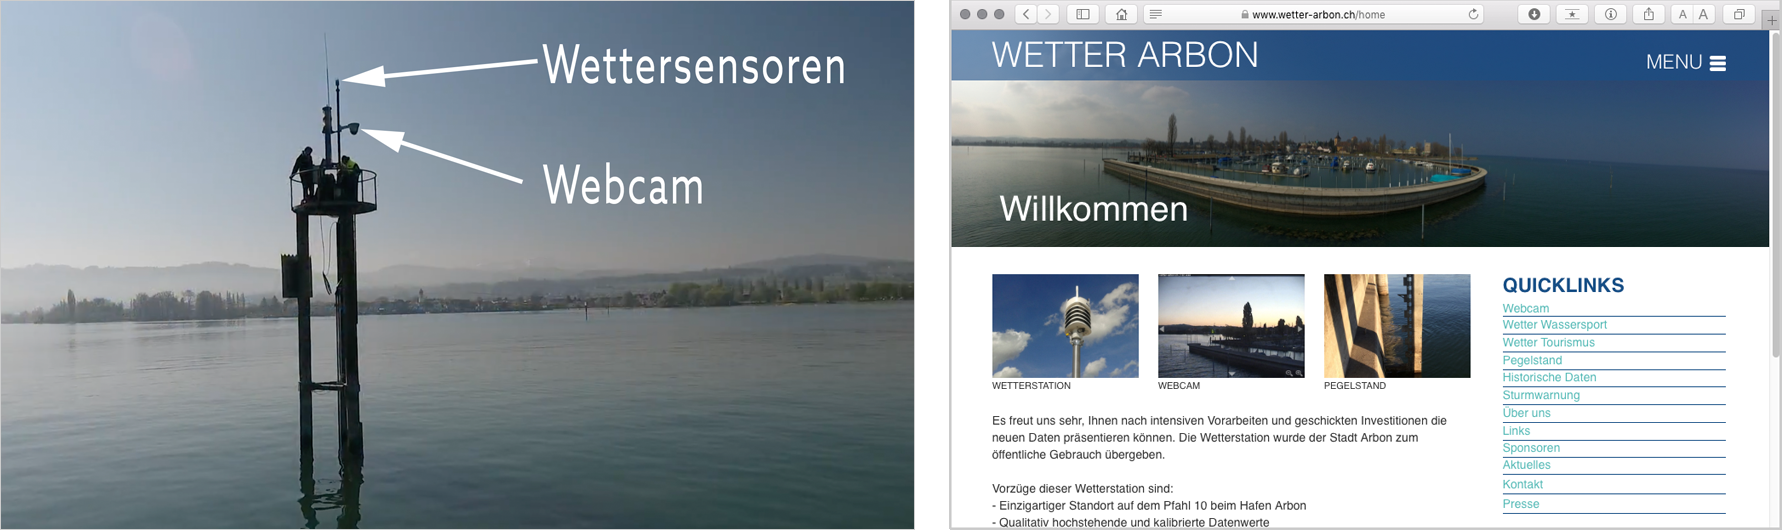
\includegraphics[width=1\linewidth]{img/kombi}
	\caption{Installation und Webseite der Wetterstation Arbon}
	\label{img:wetterstation}
\end{figure}

Was damals modern war, ist heute veraltet. Sowohl auf der Hardwareseite, als auch auf der Webseite gibt es diverses Reparatur- beziehungsweise Modernisierungspotential. Die Bachelor-Arbeit hat das Ziel die Wetterstation wieder auf einen modernen, vollfunktionsfähigen Stand zu bringen. Während des Fachmoduls, welches die Vorbereitung für die Bachelor-Arbeit darstellt, führten wir eine Ist-Aufnahme der Wetterstation Arbon durch. Im Fokus lag sowohl die Hardware als auch die Software. Der Übersicht halber und damit wir die Arbeiten besser untereinander aufteilen konnten, haben wir die Themen in die vier Blöcke:  Webseite, Datenbank, Sensoren und Webcam unterteilt. (vgl. Abb. \ref{img:module})

\vspace{5mm} %5mm vertical space

\begin{figure}[h!]
	\centering
	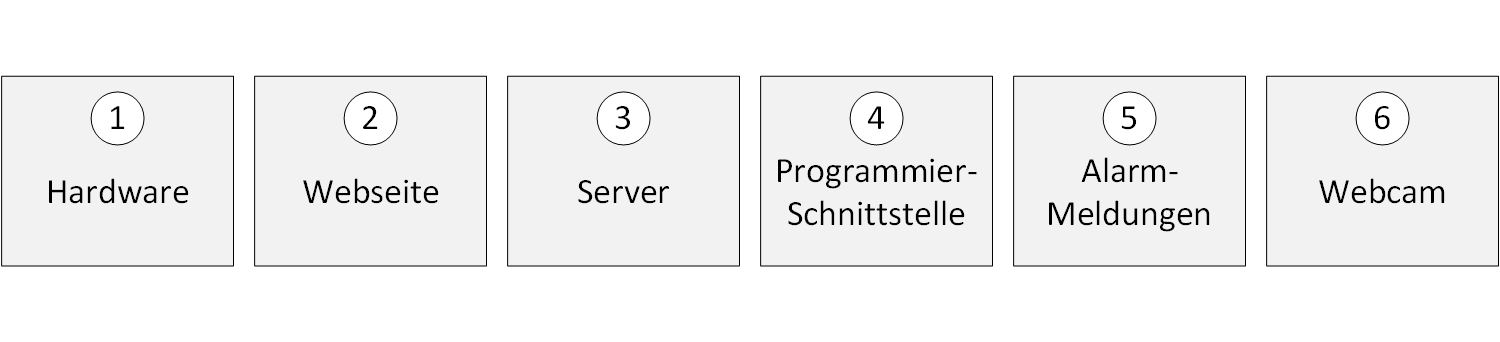
\includegraphics[width=0.8\linewidth]{img/module}
	\caption{Aufteilung in Arbeitsblöcke}
	\label{img:module}
\end{figure}

Dieser Bericht zeigt jeweils pro Block auf, wie die jetzige Situation ist, wo die Problemstellen liegen, wie diese behoben werden können und was die Anforderungen an die Lösung ist. Die Erkenntnisse des Fachmoduls dienen als Grundlage für die Bachelor-Arbeit. Dort geht es darum die Lösungsansätze zu konkretisieren und umzusetzen.

\newpage
\section*{Zusammenfassung}
\Diskussionspunkt{- Kapitel muss noch erstellt werden}\newline
\Diskussionspunkt{- Schlussfolgerung / Aussichten / weitere Schritte}\newline
\Diskussionspunkt{- Was waren die grössten Herausforderungen / was könnte besser gemacht werden}\newline
\Diskussionspunkt{- Was konnte umgesetzt werden}\newline
\Diskussionspunkt{- Welche Anforderungen wurden nicht erfüllt}\newline

\section{Datenbank}

\Diskussionspunkt{Beginn Einlesen in DB}
Verschiedene Arten von Datenbanken:
\begin{itemize}
\item relationale DB
\item hierarchisches Datenmodell
\item Netzwerkdatenmodell
\item Objekt relationale Datenbank
\end{itemize}

Das relationale Datenmodell ist das weit verbreitetste Modell, dass hierarchische wegen der beschränkten Anwendbarkeit kaum noch vorhanden.

Vorgehen Datenbankentwicklung:

\begin{itemize}
\item Externe Phase (Ermittlung der Informationsstruktur)
\item Konzeptionelle Phase (ER-Modell)
\item Logische Phase (relationales Datenmodell)
\item Physische Phase (Erstellung des Datenmodell)
\end{itemize}

Punkte zur Überlegung neuer Datenbankstruktur:
\begin{itemize}
\item Welche Daten?
\item In welchem Intervall?
\item Welche Tabellen? (Welche Daten zusammen?, eine grosse Tabelle?)
\item Tabellennamen?
\item 
\end{itemize}

Datentypen angeschaut auf w3schoolss:
\begin{itemize}
\item Welcher Datumstyp?

\end{itemize}


Unterschied MariaDB und MySQL?\\
Wie viele Daten werden gespeichert?\\
Vor der Neukonzipierung werden täglich 1440 Datensätze gespeichert. Das bedeutet jede Minute einen Datensatz. Ein Datensatz beinhaltet 65 Einträge. Die gesamte relevante Datenbank igwetter wettertest benötigt 323.17  Mb. Die Tabelle wx data benötigt stand 1.3.18 311.94 Mb, daraus erfolgt das ein Datensatz ca 0.025 Mb benötigt \\
-Wie viele Daten können gespeichert werden?\\
Die igWetter hat bei Hostpoint einen Server mit 50 GB Speicherplatz, rechnet man die vorhergehenden Zahlen hoch mit dem zur Verfügung stehenden Speicherplatz, hat es genügend Platz für die kommenden 45 Jahren.\\

https://entwickler.de/online/datenbanken/datenbanken-grundlagen-und-entwurf-115676.html
\Diskussionspunkt{Ende Einlesen in DB}\\
\Diskussionspunkt {Beginn Einlesen DB Sicherheit}\\

Bei der Recherche nach Datenbanksicherheit taucht immer wieder das Wort Injection auf. Laut den OWASP top 10, eine Liste welche die wichtigsten Schwachstellen aufzeigt, ist die SQL-injection in 2017 auf dem Platz 1. Was ist den eigentlich SQL Injection? SQL injection ist eine Methode eine Datenbankabfrage so zu manipulieren, dass der Angreifer im schlimmsten Fall auf die gespeicherten Daten des Administators kommt. Ein anderes Beispiel wäre, dass der Angreifer an die Daten der Benutzer eines Online-Shops mit Kreditkartendaten oder ähnlichen sensitiven Daten kommt.
Weitere Fragen die auftauchen bei der Suche nach Datenbanksicherheit sind:
\begin{itemize}
\item Was für Arten von Daten beherbergt die Datenbank?
\item Hat es sensitive Daten?
\item Ist die Datenbank überhaupt ein potentielles Angriffsziel?
\item Wer sind die Benutzer der Datenbank?
\end{itemize}
Neben dem Schutz vor potentiellen Angriffen ist auch der Schutz vor Datenverlust wichtig. Dieser Schutz kann sehr einfach durch ein Backup der Datenbank umgesetzt werden. Jedoch stellen sich auch hier folgende Fragen:
\begin{itemize}
\item Welche Daten sind wichtig?
\item Wie wird das Backup umgesetzt?
\item Wie oft wird ein Backup gemacht?
\end{itemize}

\Diskussionspunkt{Ende Einlesen DB Sicherheit}\\
\Diskussionspunkt{Beginn Konzept DB Sicherheit}
In der Ausgangslage der Wetterstation und deren Datenbank wird kein Backup erstellt und ist gegen aussen nicht gesichert. Wichtig hierbei ist aber zu erwähnen, dass die Datenbank im Moment ein "Datenfriedhof" ist. Die Aufgezeichneten Daten werden nicht benutzt. Im Verlauf der Bachelorarbeit wird sich dies aber ändern, deswegen ist es für die Datenbank ist wichtig, dass Sie gegen aussen vor potentiellen Angreifern und einem Verlust der Daten beim Provider gesichert ist. \\
Das Ziel ist es die Datenbank im Vergleich zu Kosten und Aufwand sicherer zu gestalten. Es wird erwartet das ein potentieller Angreifer nicht ohne Mühe in die Datenbank eindringen kann. Des Weiteren soll bei einem allfälligen Verlust der Daten auf dem Server eine schnelle Rekonstruktion der Datenbank inklusive Daten möglich sein, damit der angebotene Service schnellst möglich wieder zugänglich ist.\\ 
Um eine Neukonzipierung zu erstellen wurde vorher eine Recherche durchgeführt. Wobei für das Konzept und die spätere Umsetzung verschiedenste Fragen aufgekommen sind. Wenn es um den erhalt der Daten, also ein Backup geht, stellen sich folgende drei Grundlegende Fragen:
 \begin{itemize}
\item Welche Daten sind wichtig?
\item Wie wird das Backup umgesetzt?
\item Wie oft wird ein Backup gemacht?
\end{itemize}

Geht es um den Schutz gegen aussen vor potentiellen Angriffen tauchen die folgenden Grundlegenden Fragen auf: 
\begin{itemize}
\item Was für Arten von Daten beherbergt die Datenbank?
\item Hat es sensitive Daten?
\item Ist die Datenbank überhaupt ein potentielles Angriffsziel?
\item Wer sind die Benutzer der Datenbank?
\end{itemize}
Sind die obenstehenden Fragen beantwortet steht auch das Konzept.\\
Um die Datenbank auch gegen einen allfälligen Datenverlust zu sichern ist ein Backup von wichtiger Bedeutung. Im Grunde sind alle Daten welche die Wetterstation ablegt von Wichtigkeit. Dabei muss aber entschieden werden, ob ein tägliches Backup Sinn machen würde. Bezüglich des Speicherplatzes und des Aufwands, da die Wetterstation von einem Verein betrieben wird, ist es wichtig den Aufwand mit dem Ertrag zu vergleichen. Ein Backup nur auf dem Server des Providers macht technisch keinen Sinn, da es auch sein kann, dass dieser mal versagt und die Daten anschliessend für immer verschwunden sind. Deswegen ist es wichtig auch ein "externes" Backup zu erstellen. Es wird empfohlen ein wöchentliches Backup zu erstellen, dies aufgrund der Datenmengen, denn wöchentlich fallen 10080 Datensätze an. Fehlt eine Woche aufgrund eines Ausfalls ist der schaden geringer als ein monatliches oder jährliches Update.\\
Das update wird mittels eines Cronejobs, welches ein Backup-Script ausführt, auf dem Server durchgeführt. Die Daten werden anschliessend in einer Cloud nach Wahl hochgeladen. Zusätzlich wird das Backup auch auf dem gemieteten Server von Hostpoint gespeichert um einen schnelleren Zugriff zu gewährleisten. Um nicht zu viele Daten "unnötig" zu speichern, wird empfohlen die Daten der vorhergehenden Woche zu überspielen. Der Nachteil dieser Lösung sind jedoch die Kosten welche bei einer \Diskussionspunkt{Cloud} anfallen. Hierbei bewegt man sich preislich bei circa 10 Franken pro Monat.

Neben der Datensicherung in Form des Backups ist auch die Sicherheit im Betrieb massgebend. Bei der Recherche nach Datenbanksicherheit taucht immer wieder das Wort Injection auf. Laut den OWASP top 10, eine Liste welche die wichtigsten Schwachstellen aufzeigt, ist die SQL-injection in 2017 auf dem Platz 1. Was ist den eigentlich SQL Injection? SQL injection ist eine Methode eine Datenbankabfrage so zu manipulieren, dass der Angreifer im schlimmsten Fall auf die gespeicherten Daten des Administators kommt. Ein anderes Beispiel wäre, dass der Angreifer an die Daten der Benutzer eines Online-Shops mit Kreditkartendaten oder ähnlichen sensitiven Daten kommt. Auf der Seite der MariaDB, welche in unserem Fall benutzt wird, werden 5 Essentielle Praktiken für die Datenbanksicherheit aufgezählt:
\begin{itemize}
\item Schütze gegen Attacken mit einem Datenbankproxy
\item Setze ein auditing und robustes logging auf
\item Praktiziere ein strenges user account management
\item Halte die Datenbanksoftware und OS up-to-date
\item Verschlüssle sensitive Daten
\end{itemize}

Die Wetterstation Arbon enthält jedoch keine sensitiven Daten. Deswegen muss die Datenbank nicht mit der höchsten Sicherheit ausgestattet sein.  Trotzdem ist Datenbank nach der Umsetzung der Bachelorarbeit eins der Herzstücke der Wetterstation. Denn diese beinhaltet die Wetterdaten jeder Minute des Tages, des Weiteren erhält sie sich auch die historischen Daten der Wetterstation. Deswegen sollte eine gewisse Grundsicherheit der Datenbank gewährleistet werden, damit die Daten nicht manipuliert bzw. die Datenbank nicht anderweitig benutzt werden kann. Die Datenbank stellt nur in dieser Hinsicht ein potentielles Ziel dar. Benutzer der Datenbank hat es im eigentlichen Sinne nur zwei. Das ist der Administrator der Seite, sowie die Webseite. Jedoch sind die Benutzer der Seite auch Benutzer der Datenbank. Doch was haben diese direkt mit der Datenbank zu tun? Auf der zukünftigen Seite der historischen Daten, sollen die Benutzer entscheiden können von wann bis wann die Daten angezeigt werden sollen. Somit müssen diese eine Abfrage tätigen.\\
Um es den Angreifern nicht zu einfach zu gestalten sollte die Abfrage gegen Injection gesichert sein. Zusätzlich ist es sinnvoll mittels logging zu erfahren welche Anfragen getätigt wurden, sowie mittels eines Cronejobs die Datenbank auf dem neusten Stand zu halten. Beim logging soll bei einer Abweichung des Verhaltens, konkret heisst dies einer veränderten Abfrage, der Verein gewarnt werden. Dies kann mittels einer E-Mail stattfinden. Da es nur einen user account für den Verein hat ist es nötig diesen mit allen Privilegien auszustatten und hieran nichts zu ändern. Des Weiteren erhält wie erwähnt die Datenbank auch keine sensitiven Daten, womit ein verschlüsseln der Daten überflüssig wird. \Diskussionspunkt{Datenbankproxy}

\Diskussionspunkt{Zusammenfassung}

Das Konzept in einer kurzen Zusammenfassung inklusive den Punkten die zur Diskussion stehen:\\
Backup:\\
Es wird ein Backup system aufgesetzt welches sicherstellt, dass die Daten einmal auf dem Server von Hostpoint sowie auf extern in einer Cloud oder sonstigem externen Speicher gespeichert werden können. Dies wird mittels einem Script von einem Cronejob wöchentlich durchgeführt. Der Diskussionspunkt ist hierbei, welche der beiden externen Varianten wird gewählt und ob die Daten in einem kürzerem oder längerem Abstand gespeichert werden.

Datenbanksicherheit:\\
Die Datenbank soll primär gegen SQL-injection gesichert werden. Des Weiteren soll geloggt werden wann welche Anfragen stattfinden und wie diese aussehen. Sollte eine Abfrage aus dem Rahmen fallen, soll der Verein mittels E-Mail oder einer sonstigen Benachrichtigung gewarnt werden. Des Weiteren soll ein Cronejob und dem dazugehörigen Skript die Software auf dem neusten Stand halten. Bei der Datenbanksicherheit steht die Benachrichtigungsart und ein eventueller Proxy wie von MariaDB empfohlen zur Diskussion. 

   



%% ###################################################################################################
%%   Unterkapitel                                                                                                                                                                              #
%% ###################################################################################################

\section{ Web-Programmierschnittstelle (Web-API)}
Für die neue Webseite und für andere Anwender ist eine API erstellt worden. Um eine API zu entwickeln muss zuerst verstanden werden was eine API ist. Deswegen werden zu beginn folgende Fragen gestellt und beantwortet.
\begin{itemize}
\item Was ist eine API?
\item Wie wird eine API entwickelt?
\item Was ist state of the Art?
\end{itemize}

Anschliessend wird in diesem Kapitel aufgezeigt wie die API entwickelt wurde und wo diese zum Einsatz kommt.

\subsection{Was ist eine API?}
Eine API überbrückt die Schnittstellen zwischen verschiedenen Software teilen und strukturiert die dabei anfallende Datenübergabe dazwischen. Sie ermöglicht es Software zu modularisieren und die Kommunikation zu vereinfachen. Konkret heisst diess, dass die einzelnen Programmteile werden voneinander abgekapselt und kommunizieren nur über die Festgelegte API. Der Vorteil hierbei ist, das die API veröffentlicht werden kann und somit auch anderen die Möglichkeit gegeben werden kann die angebotenen Dienste mittels der API zu erhalten. Zusätzlich können so auch die einzelnen modularisierte Softwareteile unabhängig voneinander weiterentwickelt werden. Nicht zuletzt ist auch das Testen ein wichtiger Punkt, da alle Programmteile nur über die API miteinander kommunizieren sollten muss die Software auch nur in der Zusammenarbeit mit der API getestet werden.

http://www.omkt.de/api/

\subsection{Was ist state of the Art?}
Heutzutage wird darauf geschaut, dass die API nach dem RESTful Standard entwickelt wird. Da taucht die Frage auf was ist RESTful? Ein kleiner Exkurs. Representational State Transfer, auch REST genannt ist eine Möglichkeit so zu programmieren, dass eine Zustandslosigkeit herrscht. Ein beispiel dafür wäre die Abfrage zur Temperatur wie in Abb. \ref{img:Sequenzdiagramm_API}).  Dies bedeutet, dass jede Nachricht in sich geschlossen ist und alle Informationen die der Client bzw. der Server benötigt. Die Umsetzung dieser Paradigmas wird mit Hilfe des HTTP bzw. HTTPS Standard gemacht. Dafür kann REST die bekannten CRUD (Create, Read, Update, Delete) Befehle von HTTP benutzen.\\
\begin{figure}[h!]
	\centering
	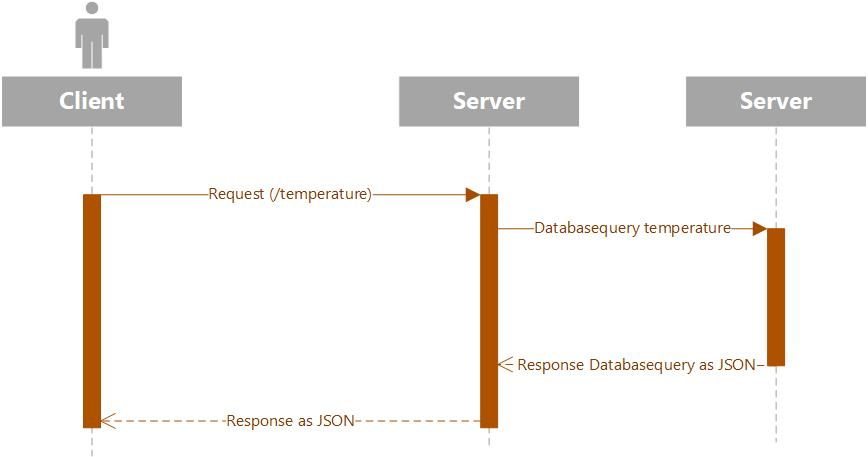
\includegraphics[width=1\linewidth]{img/Sequenzdiagramm_API}
	\caption{Beispiel einer API GET-Abfrage}
	\label{img:wetterstation}
\end{figure}

https://www.oio.de/public/xml/rest-webservices.htm

\subsection{Wie wird eine API entwickelt?}
Zu Beginn der Entwicklung muss klar sein für was die API benötigt wird. Ist dies klar, kann gesagt werden welche Anforderungen die API erfüllen muss. Als nächstes muss ein URL Schema her. Dies wird benötigt um nach dem REST Standard zu arbeiten. Die URL sollte folgendermassen aussehen: \\ https://api.wetter-arbon.ch/Versionsnummer/Endpunkt\\
Die Versionsnummer wird zur Weiterentwicklung benötigt. Wird beispielsweise eine neue Version der API veröffentlicht, kann es sein das nicht alle Nutzer der API schon auf die neue Version umgestiegen sind. Somit kann es geschehen, dass die vorhandenen Installationen zerstört werden. Neben der URL ist es wichtig das die Kommunikation in einem bestimmten Datenformat erfolgt, hier gibt es die Möglichkeit zu wählen zwischen JSON, XML oder CSV. Es können auch andere Formate genutzt werden. Wichtig ist jedoch, dass der Server sowie der Client wissen welches. Nebst der Entwicklung für die Server-Client kommunikation ist auch bei der API eine Zugangskontrolle bzw. eine Grundbasis in der Sicherheit notwendig. Neben der Möglichkeit HTTPS zu verwenden, ist es zusätzlich möglich den client über einen sogenannten Authorization Token zu zu authentifizieren. Eine andere Möglichkeit ist, den Zugriff durch eine IP-Whitelist zu begrenzen. \\

https://poe-php.de/tutorial/rest-einfuehrung-in-die-api-erstellung\\
http://edoc.sub.uni-hamburg.de/haw/volltexte/2016/3608/pdf/BAunterstrichLMauritz.pdf\\

\subsection{API Konzept}
Nachdem die Fragen zur API beantwortet sind kann die API für die Wetterstation Arbon Konzipiert und umgesetzt werden. Für die API gibt es jedoch eine wichtige Bedingung. Sie muss in php geschrieben werden, da Hostpoint kein Javascript auf der Serverseite erlaubt.

Zu Beginn des API Konzept sollten die Anforderungen daran erstellt werden. Für die Wetterstation Arbon werden folgende Anforderungen gestellt:
\begin{itemize}
\item Wind / Windrichtung
\item Niederschlag
\item Temperatur / Gefühlte Temperatur
\item Luftfeuchtigkeit
\item Wassertemperatur (1m Unter der Wasseroberfläche)
\item Wassertemperatur (Oberfläche)
\item Wasserpegel
\item Wellenhöhe
\item Radiation /daily sunduration
\item Webcam
\item Sturmwarnung
\end{itemize}
Die Datenabfrage über die API soll wie es State of the Art entwickelt wird RESTful sein und mittels HTTP geschehen. Mit der API werden nur GET-Anfragen erlaubt sein, da bspw. keine POST-Befehle oder sonstige Befehle ausgeführt werden müssen, da die API öffentlich sein soll ist auch kein Token notwendig für die Authentifizierung.

\paragraph{JSON Struktur}

Um die API zu entwickeln wurden die Anforderungen in einen sogenannten JSON-tree umgeformt. Hieraus wird auch die URL entstehen zur Abfrage der Daten. Der Aufruf wird Grundsätzlich über api.wetter-arbon.ch gemacht um einzelne Werte abzufragen muss tiefer in die Verzeichnisse gegangen werden.

\begin{lstlisting}[label=lst:Referenz,caption=Titel]
{
  "product": "api.wetter-arbon.ch",
  "version": "1.1.1",
	"v1": {
		"misc": {
			"west": {
				"description": "Warnlevel west",
				"warnlevel": 0,
				"onset": null,
				"expires": null,
				"timestamp": "2018-06-21 11:32:00",
				"interval": 60,
				"intervalUnit": "seconds"
			},
			"middle": {
				"description": "Warnlevel middle",
				"warnlevel": 0,
				"onset": null,
				"expires": null,
				"timestamp": "2018-06-21 11:32:00",
				"interval": 60,
				"intervalUnit": "seconds"
			},
			"east": {
				"description": "Warnlevel east",
				"warnlevel": 0,
				"onset": null,
				"expires": null,
				"timestamp": "2018-06-21 11:32:00",
				"interval": 60,
				"intervalUnit": "seconds"
			}
		},
		"webcam": {
			"name": "Webcam Wetter Arbon",
			"title": "webcam",
			"url": "https:\/\/webcam.wetter-arbon.ch\/mjpg\/video.mjpg"
		},
		"data": {
			"temperature": {
				"description": "Lufttemperatur",
				"unit": "\u00b0C",
				"value": 22.3,
				"dailymax": 22.7,
				"dailymin": 18.8,
				"timestamp": "2018-06-21 11:31:32",
				"interval": 60,
				"intervalUnit": "seconds"
			},
			"windchill": {
				"description": "Windchill",
				"unit": "\u00b0C",
				"value": 22.3,
				"dailymax": 22.7,
				"dailymin": 18.8,
				"timestamp": "2018-06-21 11:31:32",
				"interval": 60,
				"intervalUnit": "seconds"
			},
			"humidity": {
				"description": "Relative Luftfeuchtigkeit",
				"unit": "%",
				"value": 63,
				"timestamp": "2018-06-21 11:31:32",
				"interval": 60,
				"intervalUnit": "seconds"
			},
			"winddirection": {
				"description": "Windrichtung",
				"unit": "\u00b0",
				"value": 84,
				"timestamp": "2018-06-21 11:31:32",
				"interval": 60,
				"intervalUnit": "seconds"
			},
			"windspeed": {
				"knoten": {
					"value": 3.1,
					"dailymax": 8.6,
					"unit": "kn"
				},
				"kmph": {
					"value": 5.74,
					"dailymax": 15.93,
					"unit": "km\/h"
				},
				"beaufort": {
					"value": 2,
					"dailymax": 3,
					"unit": "Bft"
				},
				"description": "Windgeschwindigkeit",
				"timestamp": "2018-06-21 11:31:32",
				"interval": 60,
				"intervalUnit": "seconds"
			},
			"gust": {
				"knoten": {
					"value": 3,
					"dailymax": 10,
					"unit": "kn"
				},
				"kmph": {
					"value": 5.56,
					"dailymax": 18.52,
					"unit": "km\/h"
				},
				"beaufort": {
					"value": 1,
					"dailymax": 3,
					"unit": "Bft"
				},
				"description": "B\u00f6en",
				"unit": "kn",
				"timestamp": "2018-06-21 11:31:32",
				"interval": 60,
				"intervalUnit": "seconds"
			},
			"precipitation": {
				"description": "Niederschlagsmenge seit Mitternacht",
				"unit": "mm",
				"value": 0,
				"timestamp": "2018-06-21 11:31:32",
				"interval": 60,
				"intervalUnit": "seconds"
			},
			"pressure": {
				"description": "Luftdruck",
				"unit": "hPa",
				"value": 1018.3,
				"timestamp": "2018-06-21 11:31:32",
				"interval": 60,
				"intervalUnit": "seconds"
			},
			"watertemperature1m": {
				"description": "Wassertemperatur 1m unter der Wasseroberfl\u00e4che",
				"unit": "\u00b0C",
				"value": 23.8,
				"timestamp": "2018-06-21 11:31:00",
				"interval": 60,
				"intervalUnit": "seconds"
			},
			"watertemperature0m5": {
				"description": "Wassertemperatur 0.5m unter der Wasseroberfl\u00e4che",
				"unit": "\u00b0C",
				"value": 23.9,
				"timestamp": "2018-06-21 11:31:00",
				"interval": 60,
				"intervalUnit": "seconds"
			},
			"waterlevel": {
				"description": "Bodenseepegel",
				"unit": "Meter",
				"value": 4.09,
				"timestamp": "2018-06-21 11:31:00",
				"interval": 60,
				"intervalUnit": "seconds"
			},
			"radiation": {
				"radiation": {
					"description": "Globalstrahlung",
					"value": 877,
					"unit": "Watt pro Quadrameter"
				},
				"daily_sunduration": {
					"description": "Anzahl Sonnenminuten pro Tag",
					"value": 154,
					"unit": "min"
				},
				"timestamp": "2018-06-21 11:31:00",
				"interval": 60,
				"intervalUnit": "seconds"
			}
		}
	}
}

\end{lstlisting}

\subsection{Umsetzung der API}

Jetzt wo die Struktur steht kann auch das Konzept umgesetzt werden. Das Verzeichnis soll folgendermassen aufgebaut werden:

\begin{itemize}
\item Versionsnummer (V1)
\begin{itemize}
\item Data
\begin{itemize}
\item config
\end{itemize}
\item Webcam
\item misc (Verschiedenes)
\begin{itemize}
\item config
\end{itemize}
\end{itemize}
\end{itemize}

Für diesen Aufbau wurde gewählt, weil so die API erweiterbar bleibt und klar strukturiert ist. Im Verzeichnis Data werden die alle Sensordaten verarbeitet, im Verzeichnis Webcam wird nur das JSON für die Webcam erstellt, da hier keine Datenbankabfrage notwendig ist und im Verzeichnis misc werden verschiedene Daten von dritten verarbeitet.

\paragraph{PHP Files}
In diesem Unterkapitel geht es um den Grundaufbau der verschiedenen PHP Files welche im Verzeichnis Data und misc benötigt werden, zudem wird aufgezeigt wie weitere Sensordaten hinzugefügt werden können um die Modularität aufzugzeigen.
Vom Grundaufbau die Dateien im Config-Ordner alle gleich d.h ein File mit der Datenbankverbindung:
\begin{itemize}
\item path
\item database
\item databaseQuery
\item createJson
\end{itemize}

Im File Path wird die URL ausgelesen und dem richtigen Case zugewiesen. Siehe Bild. In der Zeile 21 wird die URL für den case überprüft. Ist diese richtig, wird der entsprechende Tabellenname in der dieses Attribut vorhanden ist angegeben, dies ist für die Datenbankabfrage. Anschliessend wird angegeben welche Sensorwerte aus der Datenbank benötigt werden. In Zeile 31 wird das sogenannte dataJsonStatic erstellt, hierbei wird die Beschreibung (description) und die Einheit (unit) der Daten angegeben. Grund für diesen Arraynamen ist das diese Daten statisch sind. Anschliessend wird der JSON Name vergeben in Zeile 37. Zum Schluss in Zeile wird die entsprechende Funktion im createJson aufgerufen mit der entsprechenden Parameterliste
\begin{figure}[h!]
	\centering
	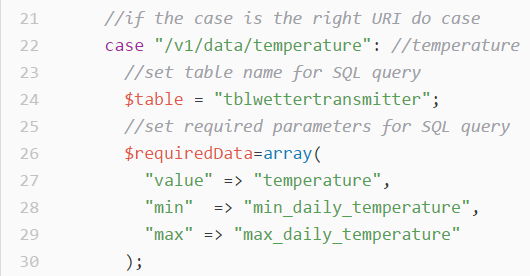
\includegraphics[width=1\linewidth]{img/API_temperature_code_path}
	\caption{Beispiel des Temperatur cases}
	\label{img:case}
\end{figure}

Nachdem die Funktion aufgerufen worden ist, geht es ins File createJson. Im File createJson bestehen verschiedene Funktionen, passend zur Anforderung. Es bestehen folgenden Funktionen welche kurz umschrieben werden welches Ziel diese haben.\\

CreateJsonMinMax:\\
Diese Funktion erstellt die JSONs mit dem aktuellen Wert sowie den Extrema des Tages.\\
CreateJson:\\
Erstellt das Json für die Daten, welche keine Extrema oder sonstige umrechnungen benötigen.
CreateJsonConversion:\\
Erstellt das Json für die Windgeschwindigkeiten mit den verschiedenen Einheiten Km/h, knoten und beufort. Umgerechnet werden die aktuellen Werte, sowie die Extrema.\\
createJsonRadiation:\\
Erstellt das Json für die Globalstrahlung zusammen mit der Sonnendauer in Minuten.\\

Zurück zum Beispiel für den Aufruf des Temperatur Jsons. In der Zeile 6 und 7 wird die Verbindung zur Datenbank hergestellt, dazu später mehr. Anschliessen wird die Klasse Sensors initialisiert und der Variable data zugewiesen und in der Zeile 8 die Datenbankabfrage durchgeführt und das Resultat in der Variablen stmt gespeichert. Nachdem die Datenbankabfrage erfolgreich wird das Resultat mittels einer while-Schlaufe in die einzelnen Spalten zerlegt und als Array gespeichert. Von Zeile 16 bis 23 wird das assoziative Array dataJson aufgebaut um in der Zeile 26 mit dem Array im File path.php zusammengefügt zu werden. Anschliessen wird das Array mittel einem echo zurückgegeben. Die restlichen Funktionen unterscheiden sich nur im Aufbau des Arrays, die Datenbankabfrage, das Aufbauen des dataJson und das Zusammenfügen sowie das zurückgeben funktioniert überall gleich.

\begin{figure}[h!]
	\centering
	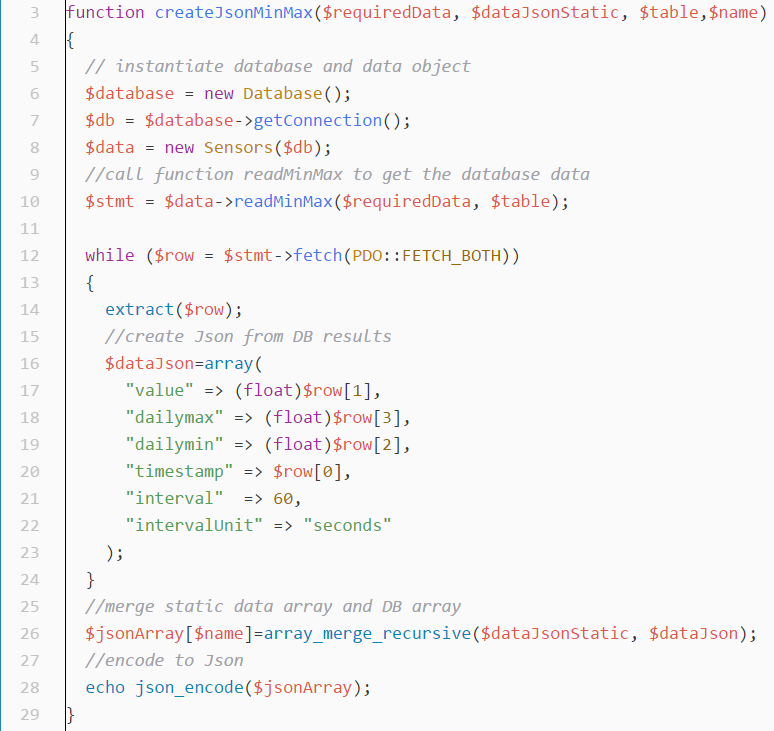
\includegraphics[width=1\linewidth]{img/API_temperature_code_createJson}
	\caption{Beispiel Erstellen des JSON}
	\label{img:wetterstation}
\end{figure}

Vor das die Datenbankabfrage ausgeführt werden kann, muss eine Datenbankverbindung hergestellt werden wie in \Diskussionspunkt{Bild} zu sehen ist. Hier wird Gebrauch vom try, catch Verfahren gemacht. Hiermit ist es möglich wie auch in anderen Programmiersprachen eine Ausnahme (Exception) abgefangen werden \cite{Ausnahmebehandlung:ThePHPGroup}. In der Zeile 21 d.h. im try wird die Verbindung durch eine Instanz der PDO Klasse erzeugt. Diese benötigt die richtigen Parameter für die Verbidung, d.h. den host, den Datenbanknamen, den Datenbankbenutzer und das Passwort.

\begin{figure}[h!]
	\centering
	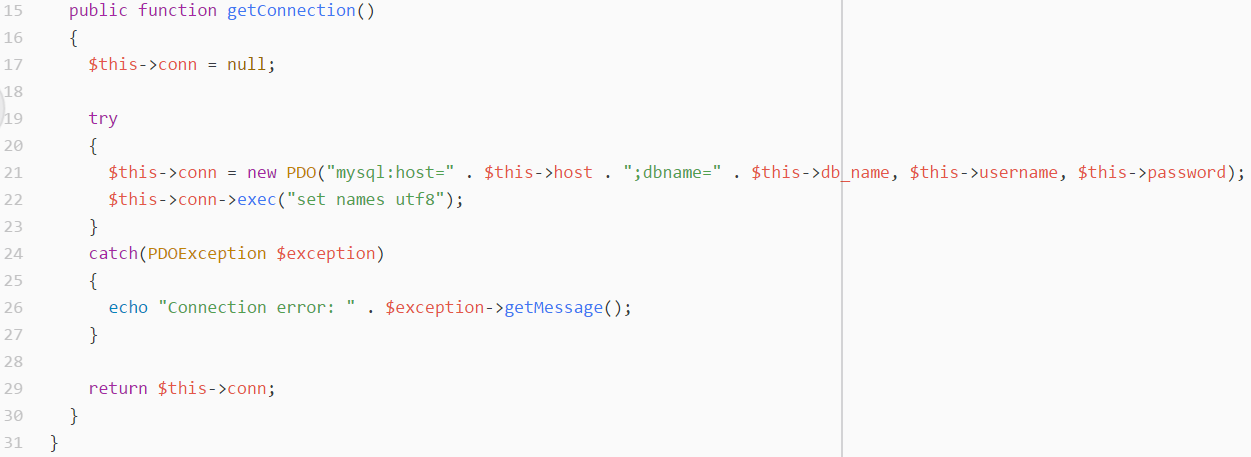
\includegraphics[width=1\linewidth]{img/API_temperature_code_database}
	\caption{Beispiel Datenbankabfrage}
	\label{img:wetterstation}
\end{figure}

Nachdem die Verbindung aufgebaut ist, wird wie bei der erklärung für das CreateJson und deren Funktion erwähnt die Datenbankabfrage durchgeführt. In Zeile 16 wird die Abrage erstellt, im Beispiel für die Temperatur würde für die variablen folgende Strings stehen:\\
\begin{lstlisting}
$requiredData['value'] -> temperature
$requiredData['min'] -> min_daily_temperature
$requiredData['max'] -> max_daily_temperature
$table ->  tblwettertransmitter
\end{lstlisting}
Diese Werte würden vorher aus der Funktion creatJsonMinMax übergeben. Ist die Query erstellt, wird diese in Zeile 20 vorbereitet und in Zeile 27 ausgeführt. Nachdem diese Ausgeführt wurde wird sie zurückgegeben an die Funktion createJsonMinMax wo die Resultate wie beschrieben aufbereitet werden zu einem Json.

\begin{figure}[h!]
	\centering
	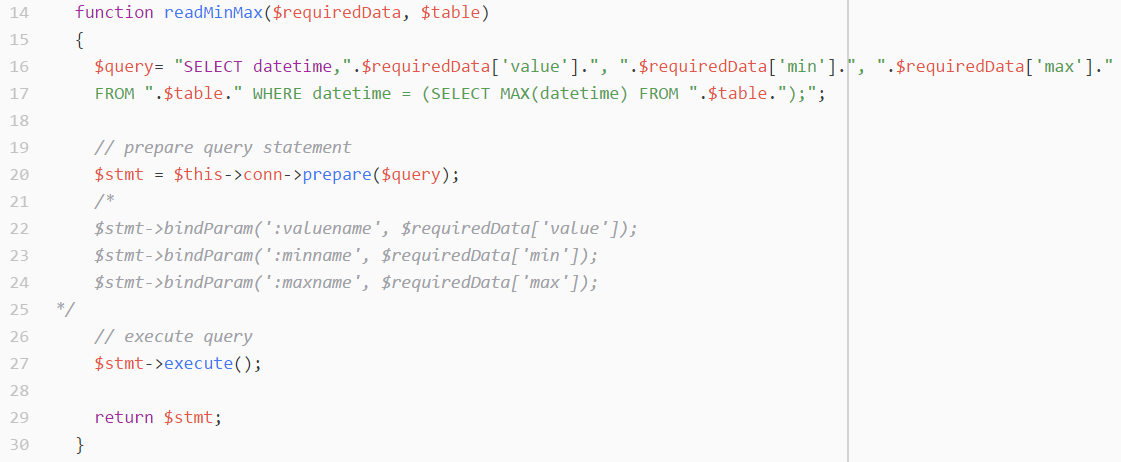
\includegraphics[width=1\linewidth]{img/API_temperature_code_databaseQuery}
	\caption{Beispiel des Temperatur cases}
	\label{img:wetterstation}
\end{figure}
 
\section{Barrierefreiheit}

Denn von einer verbesserten Zugänglichkeit profitieren nicht nur Menschen mit Einschränkungen, sondern auch die Informationsanbieter durch die Ansprache von Millionen zusätzlicher potenziellen Benutzer. Als Bonus kommt eine verbesserte Indizierung durch Suchmaschinen und infolgedessen eine bessere Position im Suchmaschinen-Ranking hinzu.

Im Kern geht es also darum, die Webapplikation so zu gestalten, dass sie möglichst für alle Benutzergruppen zugänglich ist. Dazu zählen nicht nur Menschen mit schweren und permanenten Einschränkungen, Kranke und Verletzte, funktionale Analphabeten und Legastheniker sowie die steigende Zahl an Seniorenauch veraltete Technik oder aber der allerneueste Stand der Technik (mobile Endgeräte wie etwa Tablet PC oder Smartphone) kann zu Schwierigkeiten führen.

hohen Lärmpegel (z. B. in einer Fabrikhalle) oder Zwang zur Stille (z. B. in einer Bibliothek) keine akustische Ausgabe gestatten, die Lichtverhältnisse einen besonders hohen Kontrast erfordern

Eine von Microsoft beauftragte Studie ~\cite{ForresterResearch2004E:Abilities} der \flqq Forrester Research Inc.\frqq schätzt, dass über 60 Prozent aller Computernutzer von Barrierefreiheit profitieren können. 


Gemäss \flqq Interface Design\frqq ~\cite{ThesmannStephan2016ID:U} wird Barrierefreiheit bald Standard sein.







\subsection{Web Content Accessibility Guidelines (WCAG)}

Die aktuellen Web Content Accessibility Guidelines 2.0 (WCAG2) fordern die Einhaltung von vier Designprinzipien:

\begin{itemize}  
\item Prinzip 1: Wahrnehmbarkeit 
\item Prinzip 2: Bedienbarkeit
\item Prinzip 3: Verständlichkeit
\item Prinzip 4: Robustheit
\end{itemize}

Die Ziele dieser vier Prinzipien sind durch zwölf Richtlinien (Guidelines) genauer spezifiziert. Zu jeder Richtlinie geben die WCAG2 testbare Erfolgskriterien (Success Criteria) vor.

Priorität 1 („Muss-Kriterien“): Webauftritte müssen alle A-Anforderungen erfüllen, weil es sonst für eine oder mehrere Benutzergruppen unmöglich wäre, auf die Information im Dokument zuzugreifen.

Priorität 2 („Soll-Kriterien“): Die Erfüllung der AA-Anforderungen beseitigt signifikante Hindernisse und erleichtert einer oder mehreren Benutzergruppen den Zugriff auf Web-Dokumente.

Priorität 3 („Kann-Kriterien“): Diese AAA-Anforderungen können erfüllt werden, um den Zugriff auf Web-Dokumente für eine oder mehrere Benutzergruppen zu erleichtern. Sind die Prioritäten 1 bis 3 erfüllt, erhält das Informationsangebot die Konformitätsstufe AAA.

\subsection{Relevante Anforderungen für die Webseite der Wetterstation}

\subsubsection*{Prinzip 1: Wahrnehmbarkeit}
Anforderung 1.1: Text-Alternativen 
-> für alle Anzeigegrafiken und Bilder
Anforderung 1.2: Zeitbasierte Medien 
-> Film-Aufnahme
Anforderung 1.3: Anpassbarkeit
Anforderung 1.4: Unterscheidbarkeit


\subsubsection*{Prinzip 2: Bedienbarkeit}
Anforderung 2.1: Zugänglichkeit per Tastatur
Anforderung 2.2: Bereitstellung ausreichender Zeit
Anforderung 2.3: Vermeidung von Anfällen
Anforderung 2.4: Navigierbarkeit


\subsubsection*{Prinzip 3: Verständlichkeit}
Anforderung 3.1: Lesbarkeit
Anforderung 3.2: Vorhersehbarkeit
Anforderung 3.3: Hilfestellung bei der Eingabe

\subsubsection*{Prinzip 4: Robustheit}
Anforderung 4.1: Kompatibilität


\subsection{Accessible Rich Internet Applications (WAI-ARIA) 1.1 -> Semantik}

WAI-ARIA ist eine technische Spezifikation, die ein Framework für die Verbesserung der Zugänglichkeit und Interoperabilität von Web-Inhalten und -Anwendungen bietet.

Menschen mit bestimmten Arten von Behinderungen nutzen assistive Technologien (AT), um mit Inhalten zu interagieren. Assistive Technologien können die Präsentation von Inhalten in ein für den Benutzer besser geeignetes Format umwandeln und es dem Benutzer ermöglichen, auf unterschiedliche Weise zu interagieren. Um dies effektiv zu bewerkstelligen, muss die Software die Semantik der Inhalte verstehen. Semantik ist die Wissenschaft der Bedeutung; in diesem Fall wird sie verwendet, um Rollen, Zustände und Eigenschaften zuzuweisen, die für Benutzeroberflächen und Inhaltselemente gelten, wie sie ein Mensch verstehen würde. Rollen sind eine gemeinsame Eigenschaft von accessibility APIs für die Zugänglichkeit, die von assistiven Technologien verwendet werden, um dem Benutzer eine effektive Präsentation und Interaktion zu ermöglichen.

Rollen sind Elementtypen und ändern sich nicht mit der Zeit oder Benutzeraktionen. Rolleninformationen werden von assistiven Technologien durch Interaktion mit dem User-Agent verwendet, um eine normale Verarbeitung des angegebenen Elementtyps zu ermöglichen. Zustände und Eigenschaften werden verwendet, um wichtige Attribute eines Elements zu deklarieren, die die Interaktion beeinflussen und beschreiben. 

Schlagwörter:
accessibility APIs
WAI-ARIA Roles
WAI-ARIA States and Properties

Roles:
Hauptindikator des Typs. Diese semantische Assoziation ermöglicht es den Werkzeugen, die Interaktion mit dem Objekt in einer Weise darzustellen und zu unterstützen, die mit den Erwartungen der Benutzer an andere Objekte dieses Typs übereinstimmt.

Properties:
Attribute, die für die Beschaffenheit eines bestimmten Objekts wesentlich sind oder einen mit dem Objekt verknüpften Datenwert repräsentieren. Eine Änderung einer Eigenschaft kann die Bedeutung oder Präsentation eines Objekts erheblich beeinflussen.


States:
Ein Zustand (state) ist eine dynamische Eigenschaft, die Eigenschaften eines Objekts ausdrückt, die sich als Reaktion auf Benutzeraktionen oder automatisierte Prozesse ändern können. Zustände haben keinen Einfluss auf die essentielle Natur des Objekts, sondern stellen Daten dar, die mit dem Objekt verbunden sind, oder Möglichkeiten der Benutzerinteraktion.

\Diskussionspunkt{https://www.w3.org/TR/wai-aria/#ua_noninterference}

\section{Kapitel4}
\section{Kapitel5}   
\section{Projektmanagement}
Wir wollen das Projektmanagement schlank halten um möglichst viel Zeit in die Entwicklung der Artefakte stecken zu können.
Dieser Grundgedanke hat uns bei der im Folgenden beschrieben Auswahl der Modelle und Prozesse geleitet.

% ################################
% Vorgehensmodell
% ################################
\subsection{Vorgehensmodell}

Die Anforderungen an das Vorgehensmodell haben wir folgendermassen definiert:
\begin{itemize}  
\item wenig administrativer Aufwand, schlank
\item passend zur Projektgrösse
\item kompatibel mit den NTB-Vorgaben (Aufteilung Fachmodul, Bachelor-Arbeit)
\end{itemize}

Schnell merkten wir, dass die heutzutage beliebten agilen Vorgehensmodelle wie XP oder Scrum für uns ein Overkill darstellen und aus mehrerer Hinsicht nicht geeignet sind. Bei der Bachelor-Arbeit sind die Anforderungen im Fachmodul-Bericht definiert und ändern sich während der Bachelor-Arbeit nicht mehr. Die zu bearbeitenden Themen-Blöcke weisen untereinander nur sehr wenige Schnittstellen auf und können dadurch als eigenständige Teilprojekte das Modell durchlaufen. Unser Team besteht zudem nur aus zwei Personen, was den Koordinationsaufwand auf ein minimum reduziert.

\begin{figure}[htbp]
	\centering
	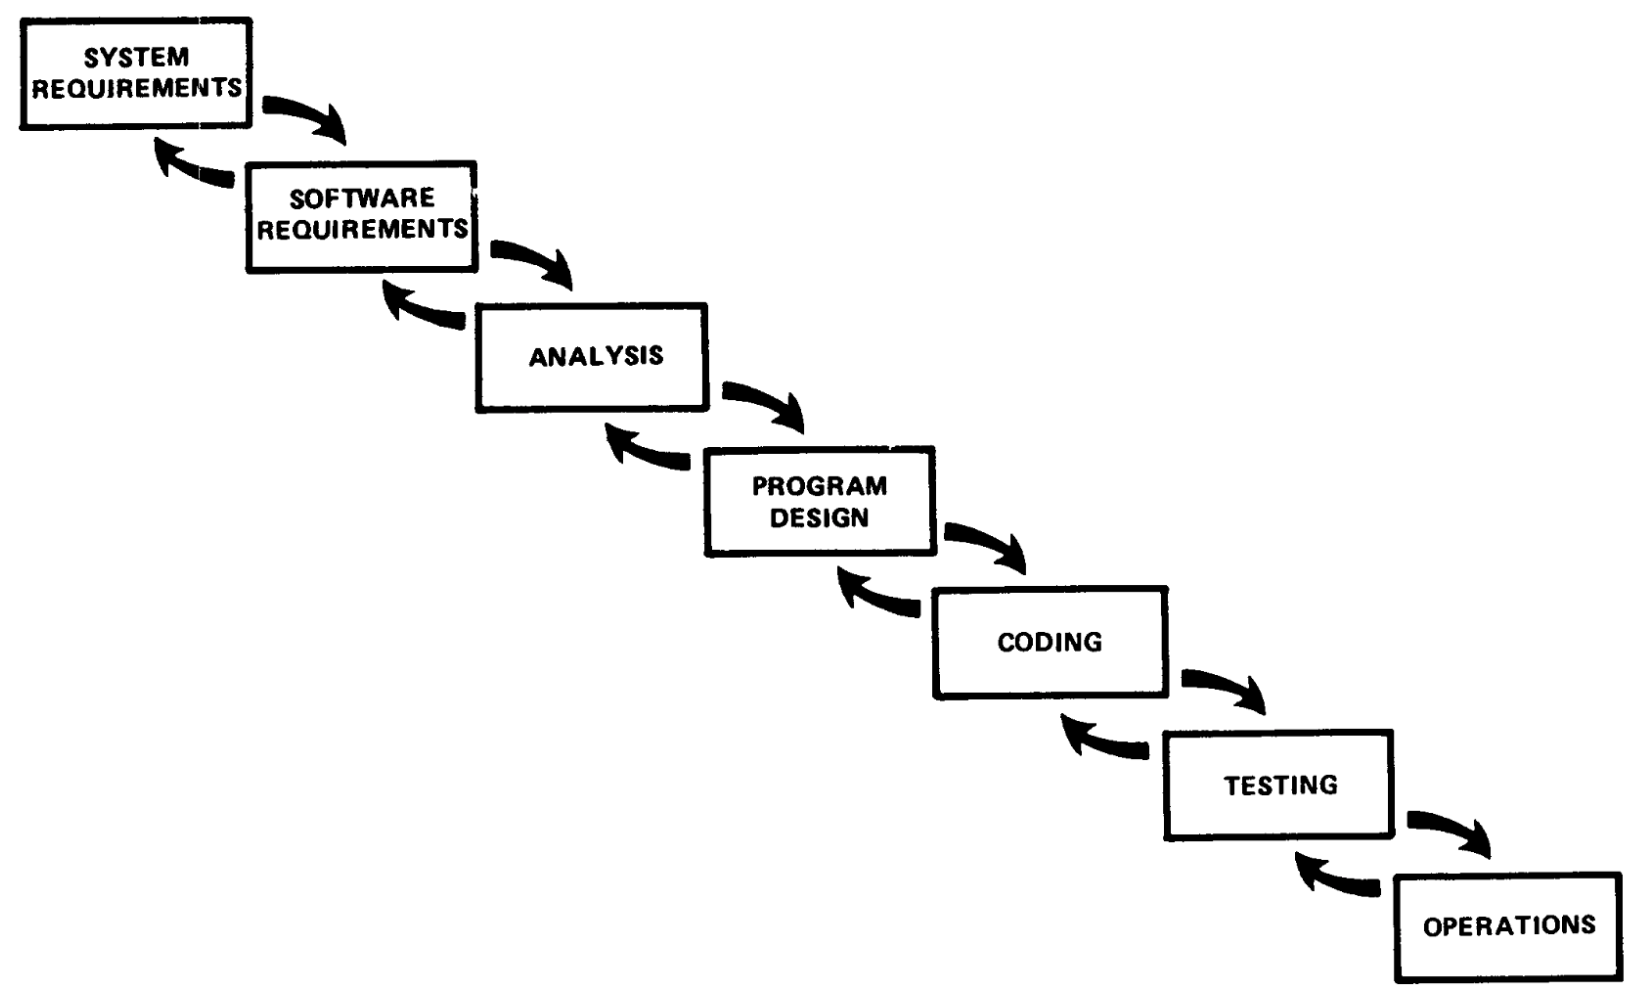
\includegraphics[width=0.9\linewidth]{img/royce-largePrograms}
	\caption{Vorgehensmodell nach Royce}
	\label{img:royce-largePrograms}
\end{figure}


Unsere Bedürfnisse deckt das Vorgehensmodell von Royce ~\cite{Royce1970}, welches in Abbildung  \ref{img:royce-largePrograms} dargestellt ist, am besten ab. Es besteht grundsätzlich aus einem sequentiellen Ablauf der Entwicklungsphasen, berücksichtigt dabei aber auch die Notwendigkeit von Rücksprüngen zur vorherigen Phase.
Die ersten Phasen von der Definition der \textit{System Requirements} bis zu den ersten Gedanken zum Thema \textit{Program Design} behandeln wir im Fachmodul. Der zweite Teil mit der genauen Definition des \textit{Programm Designs} bis zum Betrieb der Software findet anschliessend während der Bachelor-Arbeitszeit statt.


% ################################
% Entwicklungsprozess
% ################################
\subsection{Entwicklungsprozess}
Den Entwicklungsprozess führen wir mit Kanban. Kanban basiert auf dem Pull-Prinzip d.h. jeder, der im Projekt arbeitet, holt sich selbst einen neuen Arbeitsauftrag, sobald er mit einem fertig ist. Die führt dazu, dass die Arbeiten speditiver abgewickelt werden und spart zudem die Stelle des Projektmanagers, der die Aufgaben verteilt.

\begin{figure}[htbp]
	\centering
	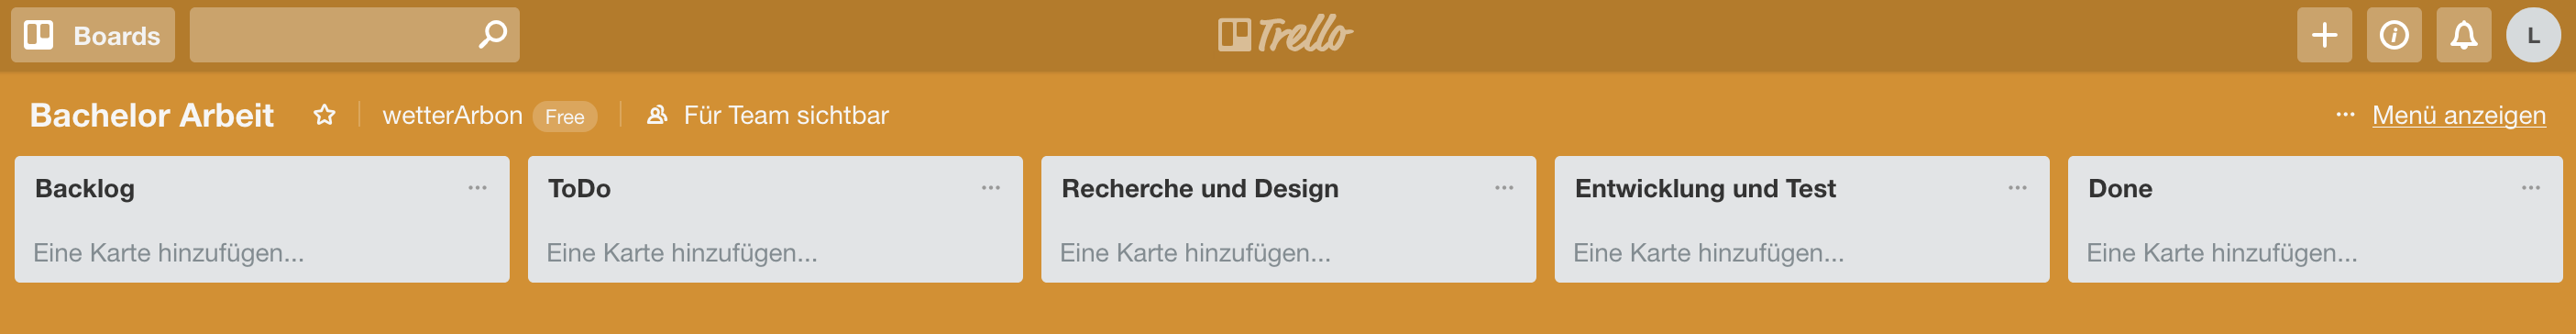
\includegraphics[width=1\linewidth]{img/kanban}
	\caption{Kanban}
	\label{img:kanban}
\end{figure}


David Anderson \cite{AndersonDavidJ2011K:eC} hat das System Kanban, welches ursprünglich aus der Industrie kommt, auf die IT angepasst und dadurch das \textit{Virtuelle Kanban System} entwickelt. Die grundlegenden Regeln daraus lauten:

\begin{itemize}  
\item Jede Karte ist eine Aufgabe
\item Die Aufgabe soll maximal 8 bis16~h benötigen
\item Pro Arbeits-Spalte sind die Anzahl Karten limitiert
\item Eine neue Karte darf erst gezogen werden, wenn die vorherige fertig ist (Multitasking-Vermeidung)
\end{itemize}

% ################################
% Risikoanalyse
% ################################
\subsection{Risikoanalyse}
Für die Risikoanalyse haben wir eine Liste der möglichen  Risiken erstellt. Als Grundlage verwendeten wir das Risikolexikon aus dem Buch \flqq IT-Risikomanagment leben!\frqq ~\cite{AhrendtsFabian2008Il:w}. 
Für jedes Risiko haben wir die Eintretenswahrscheinlichkeit und das Ausmass abgeschätzt. Gegenüber den herkömmlichen Risikobeurteilungen, haben wir allerdings die Auswirkungen auf Kosten und Terminverzug weggelassen, da sie in unserem Projekt nicht relevant sind und uns auf den Stundenaufwand und den Funktionsumfang beschränkt. Um die Auswirkung der einzelen Risiken abschätzen zu können, haben wir eine Punkteskala mit entsprechenden Kriterien erstellt, wie in Tabelle \ref{tab:auswirkung} aufgeführt. \vspace{5mm} %5mm vertical space

\begin{table}[h!]
\centering
\label{tab:auswirkung}
\begin{tabular}{rl}
Wert	[-]	& 	Auswirkung bezüglich Umfang \\
\hline
10	&	Gesamter Block nicht funktionsfähig \\
8	&	Einzelne Funktion nicht umgesetzt  \\
6	&	Bemerkbar, keine Funktionseinbusse \\
4	&	von eingeschränkter Benutzergruppe bemerkbar \\
2	&	von Kunden nicht bemerkbar
\end{tabular}
\end{table}

Die Risikomatrix in Abbildung \ref{img:risikomatrix} zeigt auf grafische Weise wie kritisch die einzelnen Risiken aus der Risikoliste sind. Mindestens vier davon sind als hoch eingestuft und müssen im Rahmen der Bachelor-Arbeit reduziert werden. Dies sind:

\begin{itemize}  
\item Komplexe Datenmigration
\item Mangel an Echtzeitverhalten
\item Mangelnde Ressourcenverfügbarkeit
\item Mangelnde Anforderungsqualität
\end{itemize}


% Abbildung der Risikomatrix
\begin{figure}[h!]
	\centering
	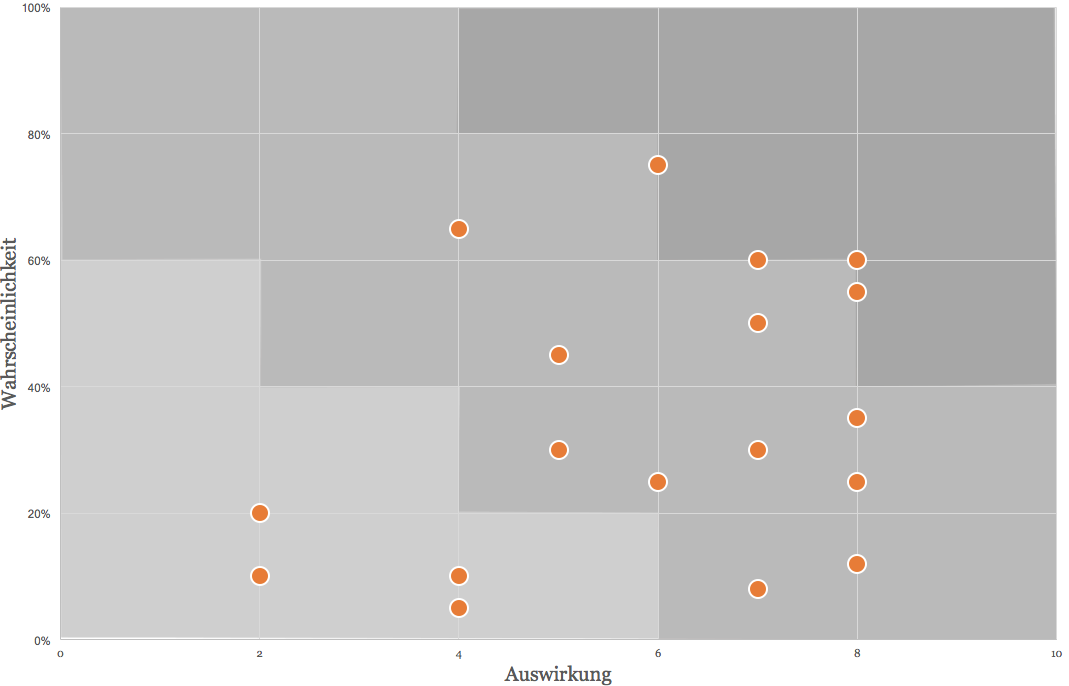
\includegraphics[width=1\linewidth]{img/risikomatrix.pdf} 
	\caption{Risikomatrix}
	\label{img:risikomatrix}
\end{figure}



% ################################
% Projektplan
% ################################

\subsection{Projektplan für die Bachelor-Arbeit}
Der Zeitplan für die Bachelor-Arbeit ist in Abbildung \ref{img:terminplan} auf Seite \pageref{img:terminplan} dargestellt.
Im oberen Teil sind die allgemeinen Termine und Abwesenheiten aufgeführt. Der mittlere Teil zeigt die Arbeitsverteilung über das Semester und am Schluss kommen die Zeitaufwände für Doku und Meetings. Die Dokumentation wollen wir kontinuierlich erstellen, sodass wöchentlich ein entsprechender Block vorgesehen ist.

\begin{figure}[h!]
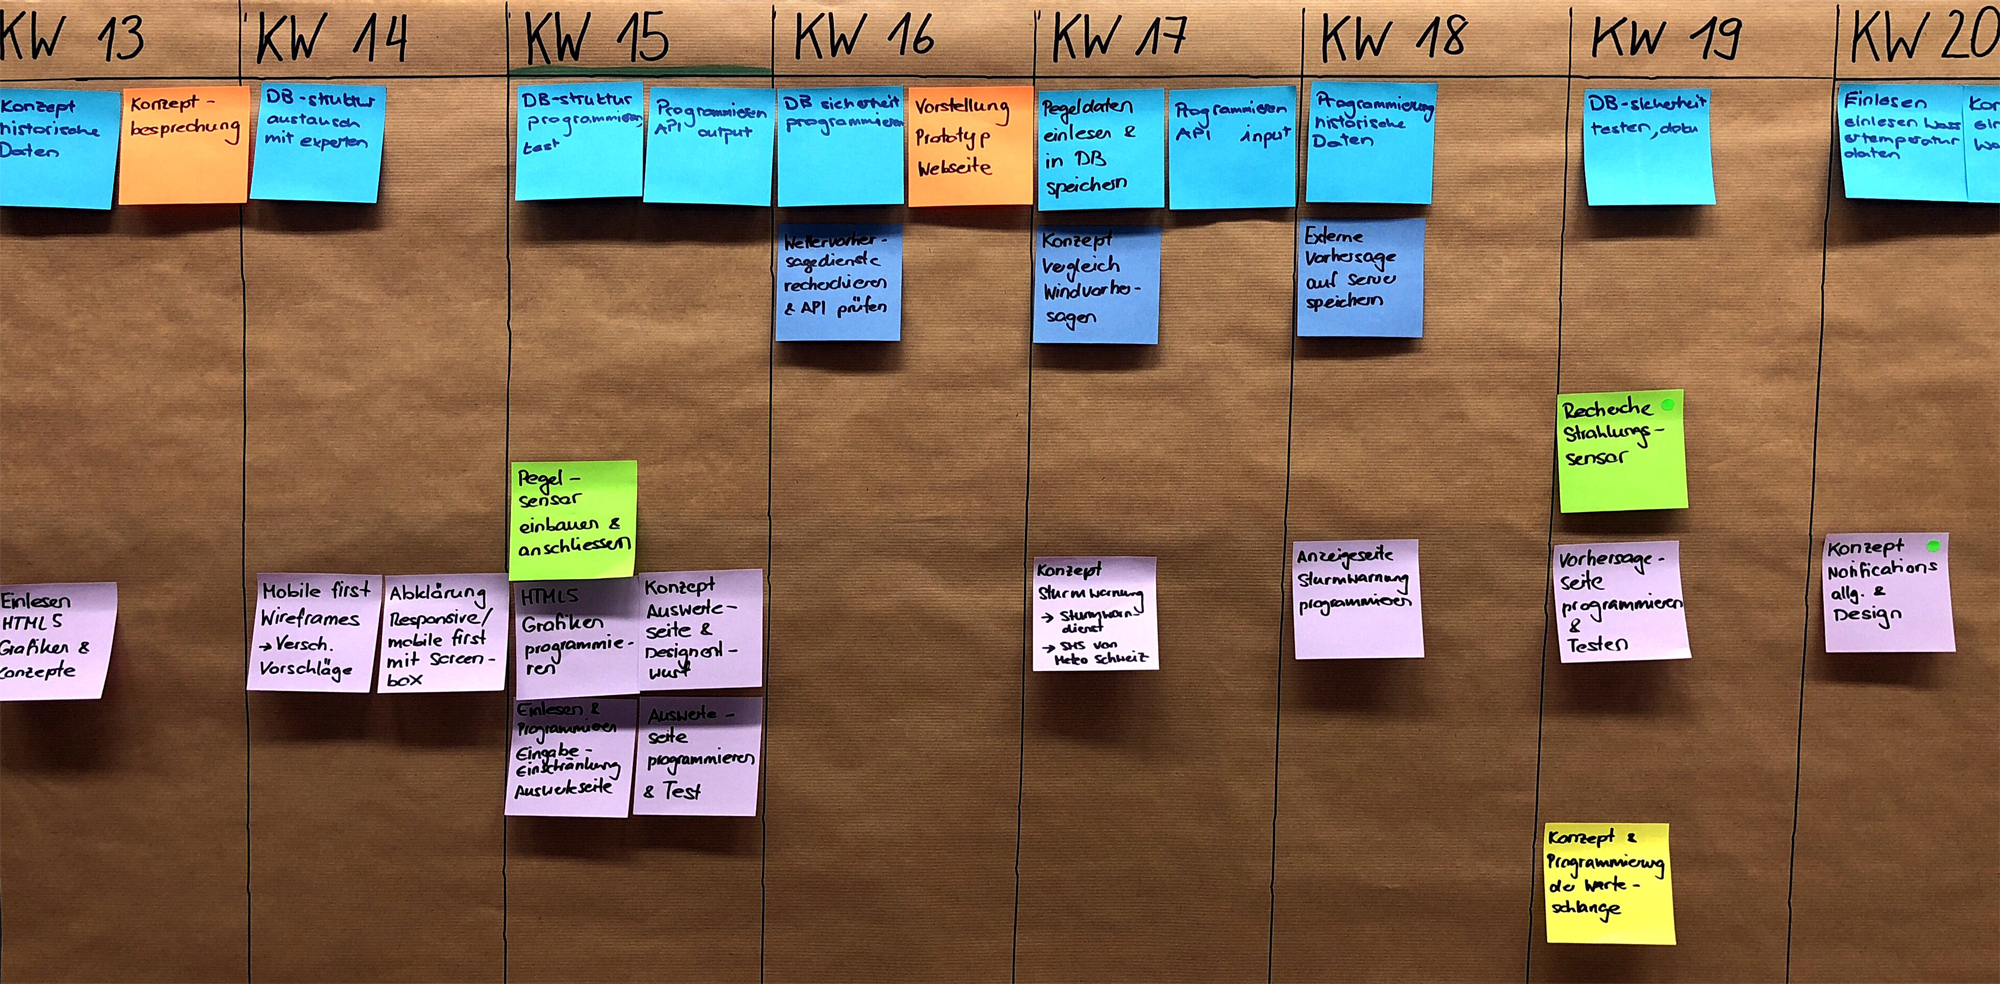
\includegraphics[angle=90,height=1\textheight,keepaspectratio]{img/terminplan.pdf}
\caption{Projektplan für die Bachelor-Arbeit}
\label{img:terminplan}
\end{figure}




\subsection{Dokumentation}

%Allgemein
Für die Bachelor-Arbeit verwenden wir unterschiedliche Dokumentationswerkzeuge. Bei der Auswahl haben wir darauf geachtet, das die Tools kostenlos nutzbar und für sämtliche Plattformen verfügbar sind (Windows, Mac, iPad, usw.). Weiter war uns wichtig, dass die Tools untereinander kommunizieren können. 

% github / Trello / Toggl
\subsubsection*{Versionierung und Zeiterfassung}
Sämtliche Artefakte speichern wir auf \textit{github}. Wir haben somit eine automatische Versionierung der Dokumente und können unabhängig voneinander an den Dokumenten arbeiten. Die Planung bzw. Darstellung des Entwicklungsprozesses erledigen wir mir \textit{Trello}. Es ist eine intuitive Webanwendung, welche diverse Integrationsmöglichkeiten mit den anderen Tools bietet. Für die Zeiterfassung verwenden wir \textit{Toggl}, welches mittels Plugin direkt in Trello integriert werden kann.

% Kommunikation nach aussen
\subsubsection*{Reporting; Kommunikation extern}
Damit wir keine Besprechungsprotokolle verschicken müssen und alle Informationen für alle immer zugänglich sind, haben wir entschieden, das Reporting in Form einer öffentlichen Webseite zu erstellen. github bietet mit \textit{GitPages} einen Hosting-Service an, der genau dies ermöglicht. Der Vorteil von \textit{GitPages} ist, dass wir sämtliche Daten in einem einzigen Ort bzw. Repository vereint haben. Damit wir uns nicht mit Formatierung herumschlagen müssen und uns auf den Inhalt konzentrieren können, verwenden wir \textit{mkdocs} als Template Engine. Die Webseiten-Einträge können wir dadurch auf simple Art in Form von Markdown-Files erstellen.

% Kommunikation nach innen
\subsubsection*{Kommunikation teamintern}
Innerhalb des Teams nutzen wir das Kommunikationstool \textit{Slack}. Dieses ermöglicht uns, Konversationen als Chat aufzuzeichnen und nach Themen zu gruppieren. Weiter lassen sich Dokumente austauschen. Sämtliche git-Posts werden von Slack automatisch geloggt und können, falls gewünscht, als push-Notification angezeigt werden.
Das wöchentliche Team-Meeting findet über \textit{Skype} statt, da wir den regelmässigen mündlichen Austausch als zentralen Punkt erachten.

% Bericht = LaTeX
\subsubsection*{Dokumentation}
Den Bericht werden wir in \LaTeX\ verfassen. Wir haben uns für \LaTeX\ entschieden, da wir uns auf den Inhalt konzentrieren können und das Layout automatisiert ist. Weiter ist \LaTeX\ in der Wissenschaft weit verbreitet. Die Bachelor-Arbeit ist deshalb eine gute Gelegenheit, uns in dieses Thema einzuarbeiten.




% braucht es das?
\FloatBarrier

\newpage
%%%%%%%%%%%%%%%%%%%%%%%%%%%%%%%%%%%
%%  Schluss
%%%%%%%%%%%%%%%%%%%%%%%%%%%%%%%%%%%
\section{Schluss}
% viele Konzepte
Während der Analyse der Wetterstation konnten wir diverse Schwachstellen ausfindig machen, die mehr oder weniger dringend beseitigt werden müssen.
Bei vielen Problemen muss zuerst ein Lösungskonzept erstellt werden, bevor mit der Behebung begonnen werden kann. Diese Arbeit bedarf einiges an Recherchearbeit und darf nicht unterschätzt werden.
\newline

\noindent
% unbekannte Thematik
Das gesamte Themengebiet von Barrierefreiheit und User Interface Design ist für uns neu und wir müssen das gesamt Know-how von Grund auf aufbauen. Ebenso ist die Arbeit mit Skripten und die Verdünnung der Daten auf einer Datenbank neu für uns. Auch hier ist ein grosser Teil für Einlesearbeiten zu erwarten.
\newline

\noindent
% schwierige Rahmenbedingungen
Als kritisch bezwiehungsweise schwer abschätzbar sehen wir die gegebenen Rahmenbedingung, die uns allenfalls in der Lösungsfindung stark einschränken.
Zum Beispiel ist dies das vorgegebene CMS oder die Schnittstelle zum Kombi-Wetter-Transmitter über \textit{WeatherDisplay}.
\newline

\noindent
% Rückblick auf Stundenschätzung
Anfangs Fachmodul schätzen wir die Stundenaufwände für die während dem Fachmodul anstehenden Arbeiten ab. Die effektiven Aufwände haben wir mittels Toggl dokumentier, sodass wir nun am Schluss des Fachmoduls die geleisteten Stunden den geplanten gegenüberstellen können. Die Auflistung befindet sich in Tabelle~\ref{plan-ist}. 
Sowohl die produktiven Arbeiten, d.h. die Arbeiten, die gemäss Fachmodul-Auftrag zu erledigen waren, als auch die Administrativen Aufwände für Meetings und Wochenreports stimmen recht gut. Der Aufwand für die Dokumentation hingegen haben wir unterschätzt. Wenn wir anfangs Bachelor-Arbeit den definitiven Terminplan erstellen müssen wir dies berücksichtigen.
\newline

\begin{table}[h]
\centering
\begin{tabular}{|l|l|l|l|}
\hline
 Tätigkeit			&  Plan	& Ist  	& Delta  		\\ \hline
 Produktive Arbeit	&  86		&  75		&  13~\%		\\ \hline
 Dokumentation		&  44		&  73		&  65~\%		\\ \hline
 Administration		&  30		&  27		&  10~\%		\\ \hline
\end{tabular}
\caption{Vergleich der Planstunden zu den Ist-Stunden}
\label{table:plan-ist}
\end{table}

\noindent
Zusammenfassend sehen wir Bachelor-Arbeit als machbar an. Zeitlich bleibt jedoch nicht viel Spielraum. Die grossen Unbekannten wie  einschränkende Rahmenbedingungen und schwer abzuschätzenden Aufwand für Einarbeitung und Konzepterstellung bedingen jedoch, dass der Fortschritt kontinuierlich und kritisch geprüft wird.
\section{Rechtliche Ansprüche}
siehe separates Dokument
\section{Verzichterklärung}
\newpage
\bibliography{literatur}{}	
\bibliographystyle{plain} 


\end{document}